\documentclass[12pt, twoside]{article}
\usepackage[letterpaper, margin=1in, headsep=0.5in]{geometry}
\usepackage[english]{babel}
\usepackage[utf8]{inputenc}
\usepackage{amsmath}
\usepackage{amsfonts}
\usepackage{amssymb}
\usepackage{tikz}
%\usetikzlibrary{quotes, angles}

\usepackage{graphicx}
\usepackage{enumitem}
\usepackage{multicol}

\usepackage{fancyhdr}
\pagestyle{fancy}
\fancyhf{}
\renewcommand{\headrulewidth}{0pt} % disable the underline of the header

\fancyhead[LE]{\thepage}
\fancyhead[RO]{\thepage \\ Name: \hspace{3cm}}
\fancyhead[L]{BECA / Dr. Huson / Geometry\\* Unit 6: Distance \& slope\\* 6 December 2019}

\begin{document}
\subsubsection*{6.8 Do Now: Euclid's Garden, mapping angles to slope}
  \begin{enumerate}

  \item This diagram is an example of what is called ``Euclid's Orchard" representing integer coordinate pairs viewed from the origin.
  \begin{enumerate}
    \item Replicate the points and angles below onto page 3.
    \item Complete the table of values on page 2 by measuring the angles with a protractor.
    \item Use your table to answer the questions on page 4.
  \end{enumerate}
  \begin{flushright}
    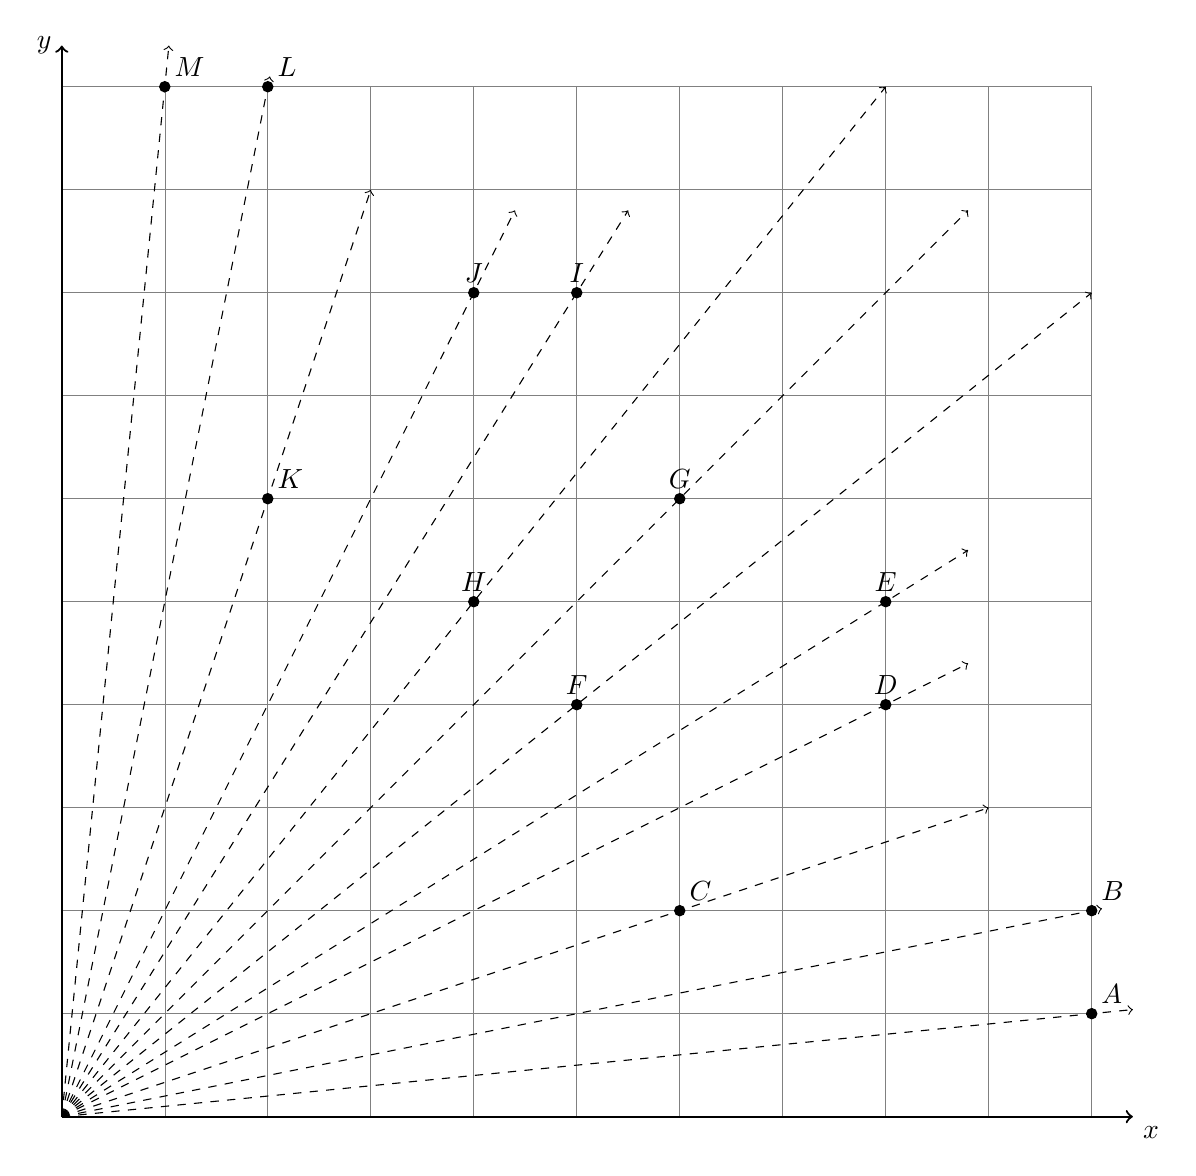
\begin{tikzpicture}[scale=1.308]
      \draw [help lines] (0,0) grid (10,10);
      \draw [thick, ->] (0,0) -- (10.4,0) node [below right] {$x$};
      \draw [thick, ->] (0,0)--(0,10.4) node [left] {$y$};
      \draw [fill] (10, 1) circle[radius = 0.05] node[above right]{$A$};
      \draw [dashed, ->] (0,0)--(10.4, 1.04);
      \draw [fill] (10, 2) circle[radius = 0.05] node[above right]{$B$};
      \draw [dashed, ->] (0,0)--(10.1, 2.02);
      \draw [fill] (6, 2) circle[radius = 0.05] node[above right]{$C$};
      \draw [dashed, ->] (0,0)--(9, 3);
      \draw [fill] (8, 4) circle[radius = 0.05] node[above]{$D$};
      \draw [dashed, ->] (0,0)--(8.8, 4.4);
      \draw [fill] (8, 5) circle[radius = 0.05] node[above]{$E$};
      \draw [dashed, ->] (0,0)--(8.8, 5.5);
      \draw [fill] (5, 4) circle[radius = 0.05] node[above]{$F$};
      \draw [dashed, ->] (0,0)--(10, 8);
      \draw [fill] (6, 6) circle[radius = 0.05] node[above]{$G$};
      \draw [dashed, ->] (0,0)--(8.8, 8.8);
      \draw [fill] (4, 5) circle[radius = 0.05] node[above]{$H$};
      \draw [dashed, ->] (0,0)--(8, 10);
      \draw [fill] (5, 8) circle[radius = 0.05] node[above]{$I$};
      \draw [dashed, ->] (0,0)--(5.5, 8.8);
      \draw [fill] (4, 8) circle[radius = 0.05] node[above]{$J$};
      \draw [dashed, ->] (0,0)--(4.4, 8.8);
      \draw [fill] (2, 6) circle[radius = 0.05] node[above right]{$K$};
      \draw [dashed, ->] (0,0)--(3, 9);
      \draw [fill] (2, 10) circle[radius = 0.05] node[above right]{$L$};
      \draw [dashed, ->] (0,0)--(2.02, 10.1);
      \draw [fill] (1, 10) circle[radius = 0.05] node[above right]{$M$};
      \draw [dashed, ->] (0,0)--(1.04, 10.4);
    \end{tikzpicture}
      \end{flushright}

    
\newpage 
\subsubsection*{Complete the table mapping slopes to angle measures}

\begin{tabular}{|l|r@{\hskip 1.5cm}r@{\hskip 1cm}rr}
  \hline
  Point & $x$ & $y$  & slope $m$ & angle measure $\theta$\\ 
  \hline 
  $A$ & 10 & 1 & 0.1 & $6^\circ$ \\[0.5cm] 
  $B$ &  &  &  &  \\[0.5cm] 
  $C$ &  &  &  &  \\[0.5cm] 
  \hline 
  $D$ &  &  &  &  \\[0.5cm] 
  $E$ &  &  &  &  \\[0.5cm] 
  $F$ &  &  &  &  \\[0.5cm] 
  \hline 
  $G$ &  &  &  &  \\[0.5cm] 
  $H$ &  &  &  &  \\[0.5cm] 
  $I$ &  &  &  &  \\[0.5cm] 
  \hline 
  $J$ &  &  &  &  \\[0.5cm] 
  $K$ &  &  &  &  \\[0.5cm] 
  $L$ &  &  &  &  \\[0.5cm] 
  \hline   
  $M$ &  &  &  &  \\[0.5cm]
\end{tabular}

\newpage
\item Add points and vertex angles to the grid below, labeling them as was done on the first page. Then complete the table on page 2, as follows:
\begin{enumerate}
  \item Write down the $x$ and $y$ coordinates of the point;
  \item Calculate the slope, ``rise over run'', as a decimal to the nearest thousandth;
  \item Measure the angle, $\theta$, made with the origin and $x$-axis, as shown for point $A$.
\end{enumerate}
\begin{flushright}
  \begin{tikzpicture}[scale=1.308]
    \draw [help lines] (0,0) grid (10,10);
    \draw [thick, ->] (0,0) -- (10.4,0) node [below right] {$x$};
    \draw [thick, ->] (0,0)--(0,10.4) node [left] {$y$};

  \end{tikzpicture}
    \end{flushright}

\newpage
Use your table of slopes and angles to answer the following questions. 
  \item A line intersects the $x$-axis at the origin at an angle of $18^\circ$. What is it's slope? \vspace{1cm}
  \item A line intersects the $x$-axis at the origin at an angle of $63^\circ$. What is it's slope? \vspace{1cm}
  \item A line through the origin has a slope of 1. What angle does it make with the $x$-origin? \vspace{1cm}
  \item Right $\triangle ABC$ has a base of length 8 and height 4. What is the measure of the vertex $\angle A$?
    \begin{flushright}
    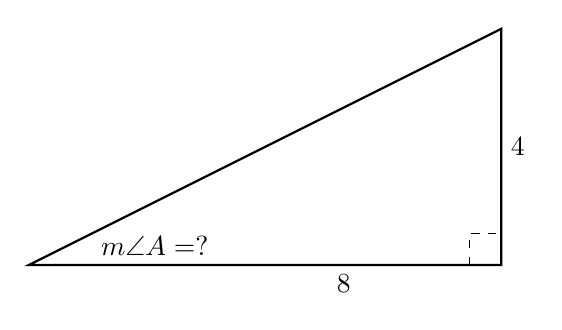
\begin{tikzpicture}[scale=1]
        \node at (1.6,0)[above]{$m\angle A=?$};
        \node at (6,1.5)[right]{4};
        \node at (4,0)[below]{8};
        \draw [thick] (0, 0)--(6, 0)--(6, 3)--cycle;
        \draw [dashed] (6,0)++(-0.4,0)-- ++(0,0.4)-- +(0.4,0);
      \end{tikzpicture}
    \end{flushright} 

    \item Right $\triangle DEF$ has a base of length 4 and height $h$. The measure of the vertex $\angle D = 51^\circ$. Find the height, $h=?$.
    \begin{flushright}
    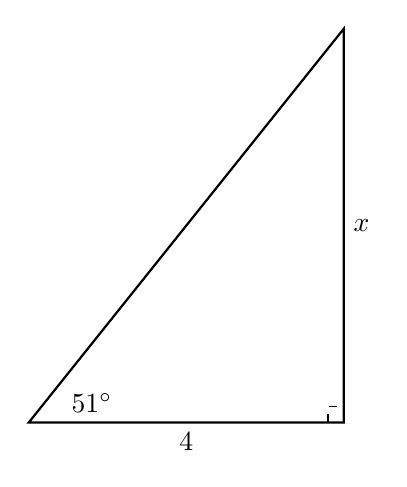
\begin{tikzpicture}[scale=0.5]
        \node at (1.6,0)[above]{$51^\circ$};
        \node at (8,5)[right]{$x$};
        \node at (4,0)[below]{4};
        \draw [thick] (0, 0)--(8, 0)--(8, 10)--cycle;
        \draw [dashed] (8,0)++(-0.4,0)-- ++(0,0.4)-- +(0.4,0);
      \end{tikzpicture}
    \end{flushright}

\end{enumerate}
\end{document}
